Når spenningen over base-emitter dioden når ca $\SI{0.7}{\volt}$
vil det gå strøm fra emitter til base.
Fra det punktet vil strømmen $I_C$ holde seg nesten konstant,
selv om $V_{CE}$ øker.

Når $V_{CE}$ øker, blir sperresjiktet tykkere.
Men hvis spenningen blir for stor får vi et \emph{punch through}.
\\\\
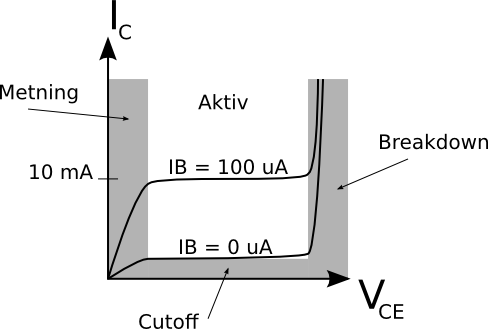
\includegraphics[width=\textwidth]{./img/npn-virkeomrade}
